\begin{figure*}[t]
    \centering
        % 第四张图：Zero-Variance Ratio
    \begin{subfigure}[b]{0.24\textwidth}
        \centering
        % \includegraphics[width=\textwidth]{figures/experiment/9-zero-variance-ratio-comparison-smoothed.png}
        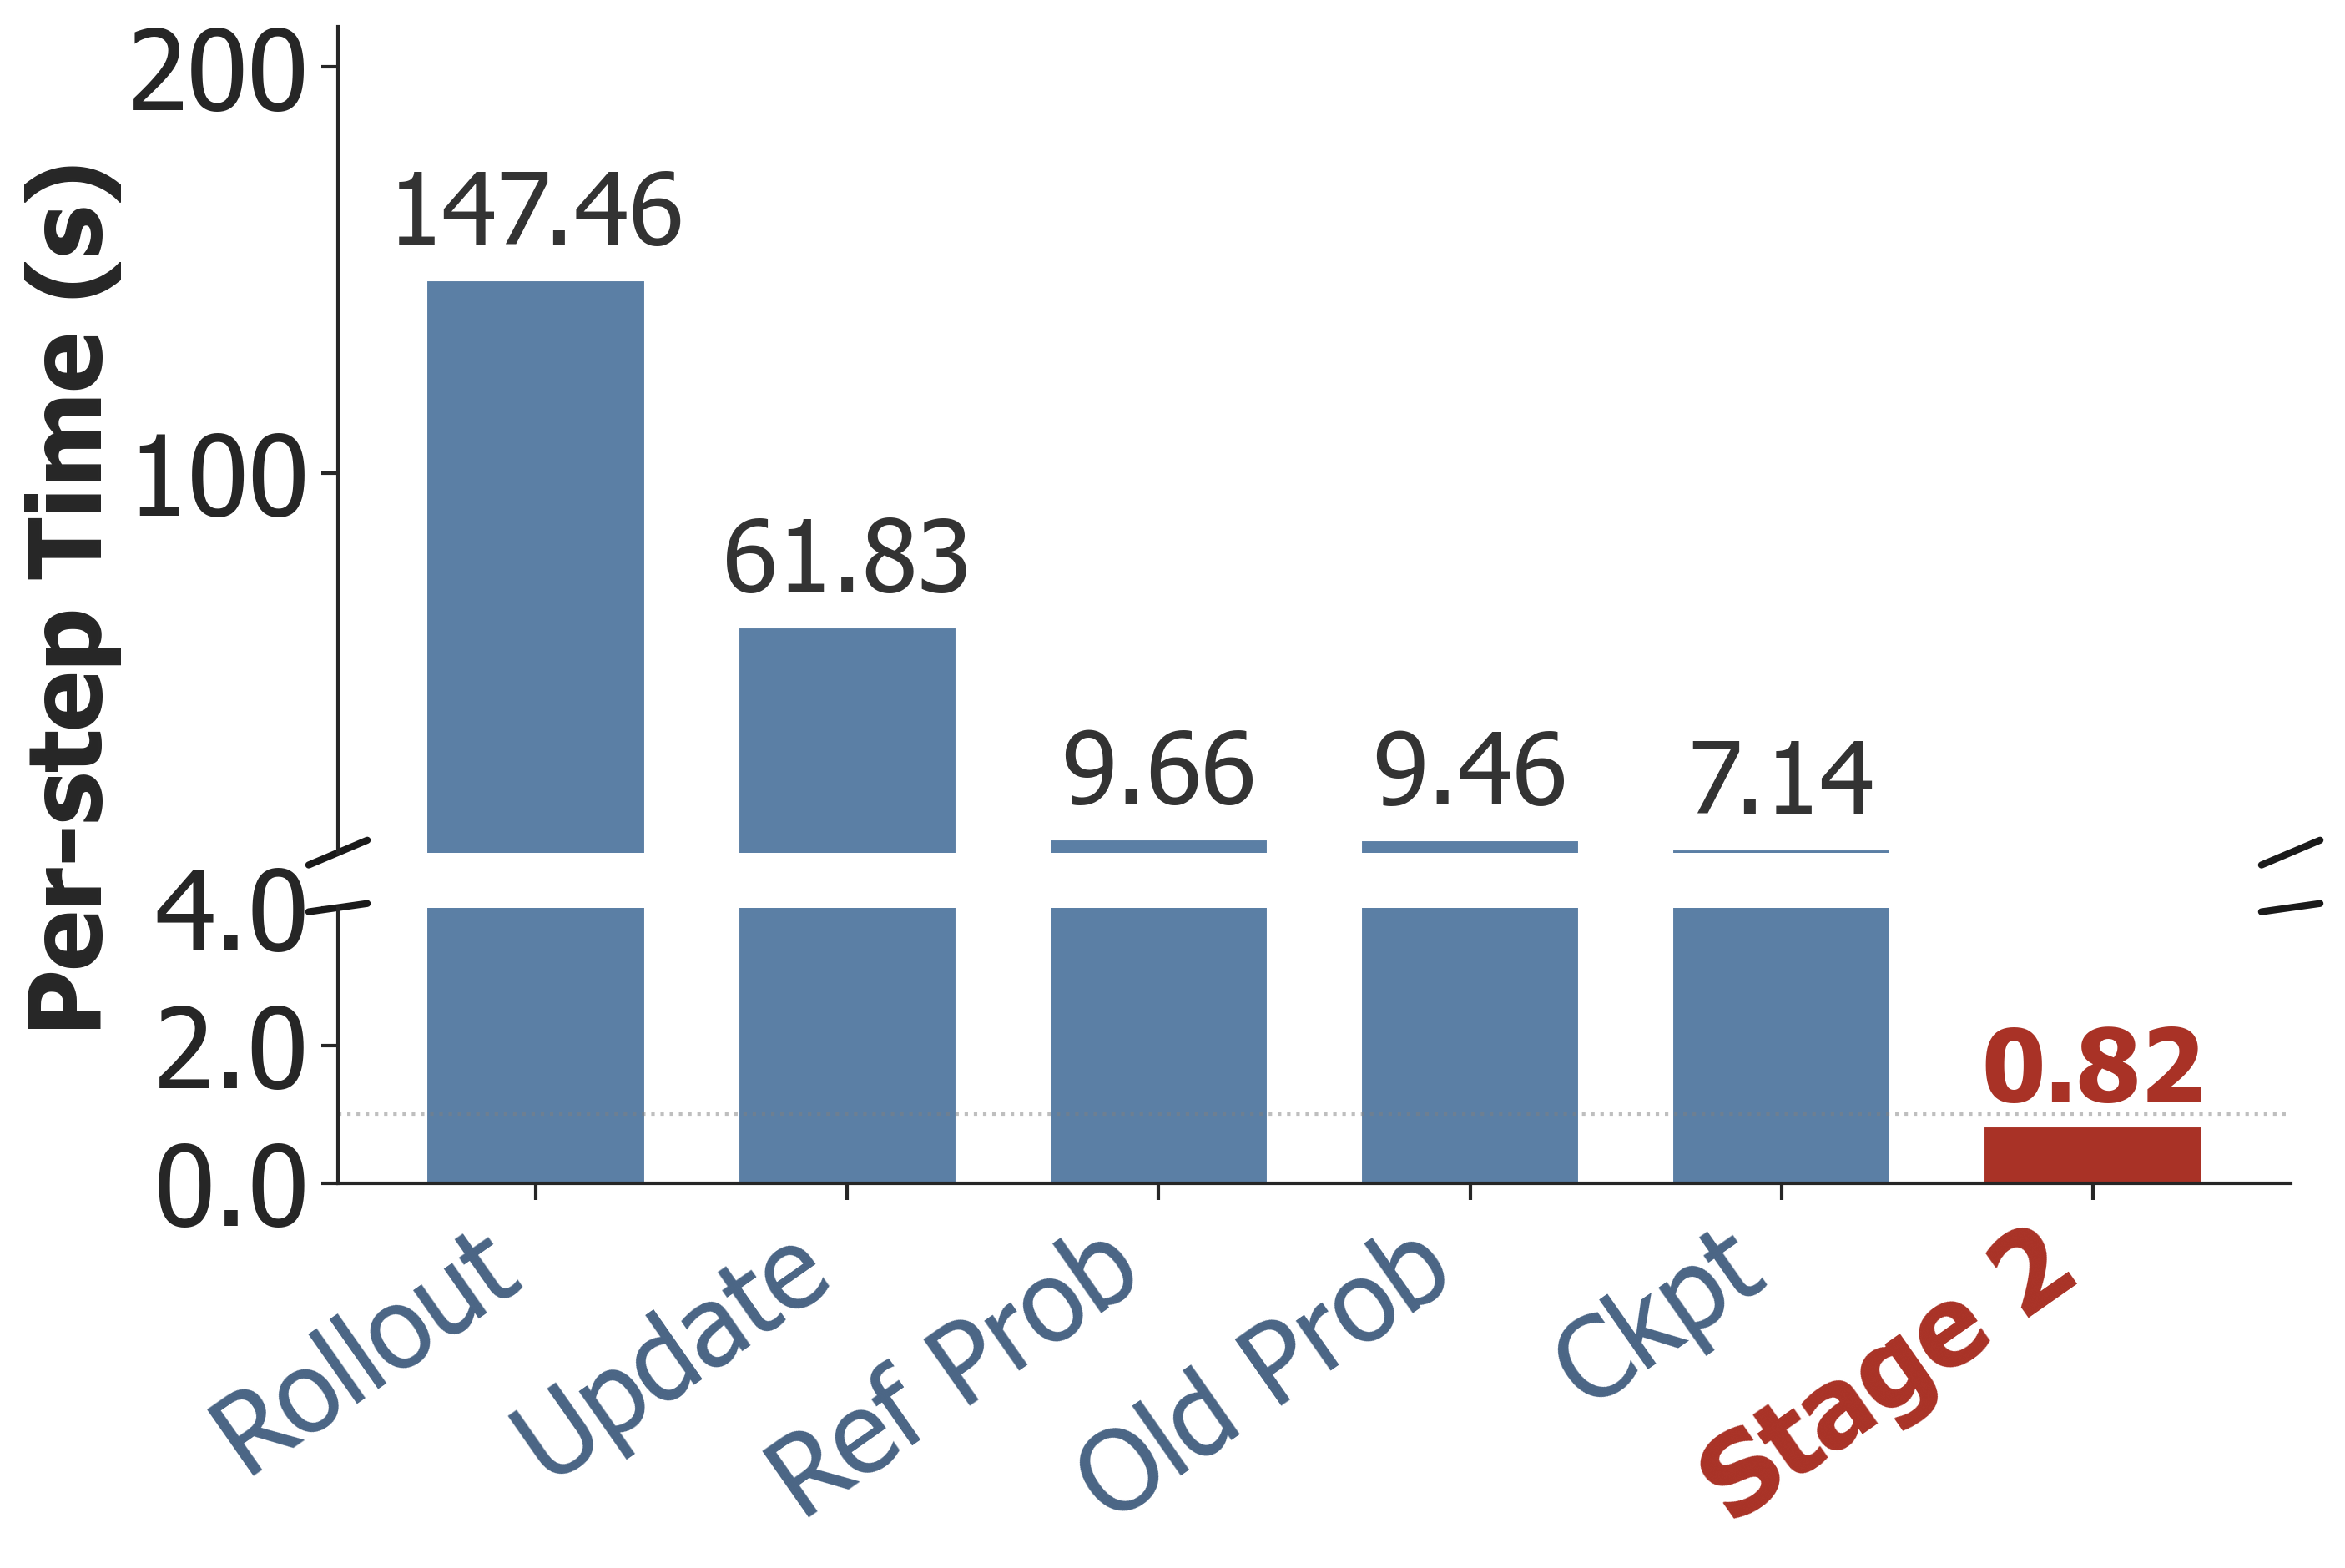
\includegraphics[width=\textwidth]{figures/experiment/5-broken_axis_styled.png}
        \caption{{Train-Time Breakdown}}
        \label{fig:per_step_time_analysis}
    \end{subfigure}
    % 第一张图：Rollout vs Time
    \begin{subfigure}[b]{0.24\textwidth}
        \centering
        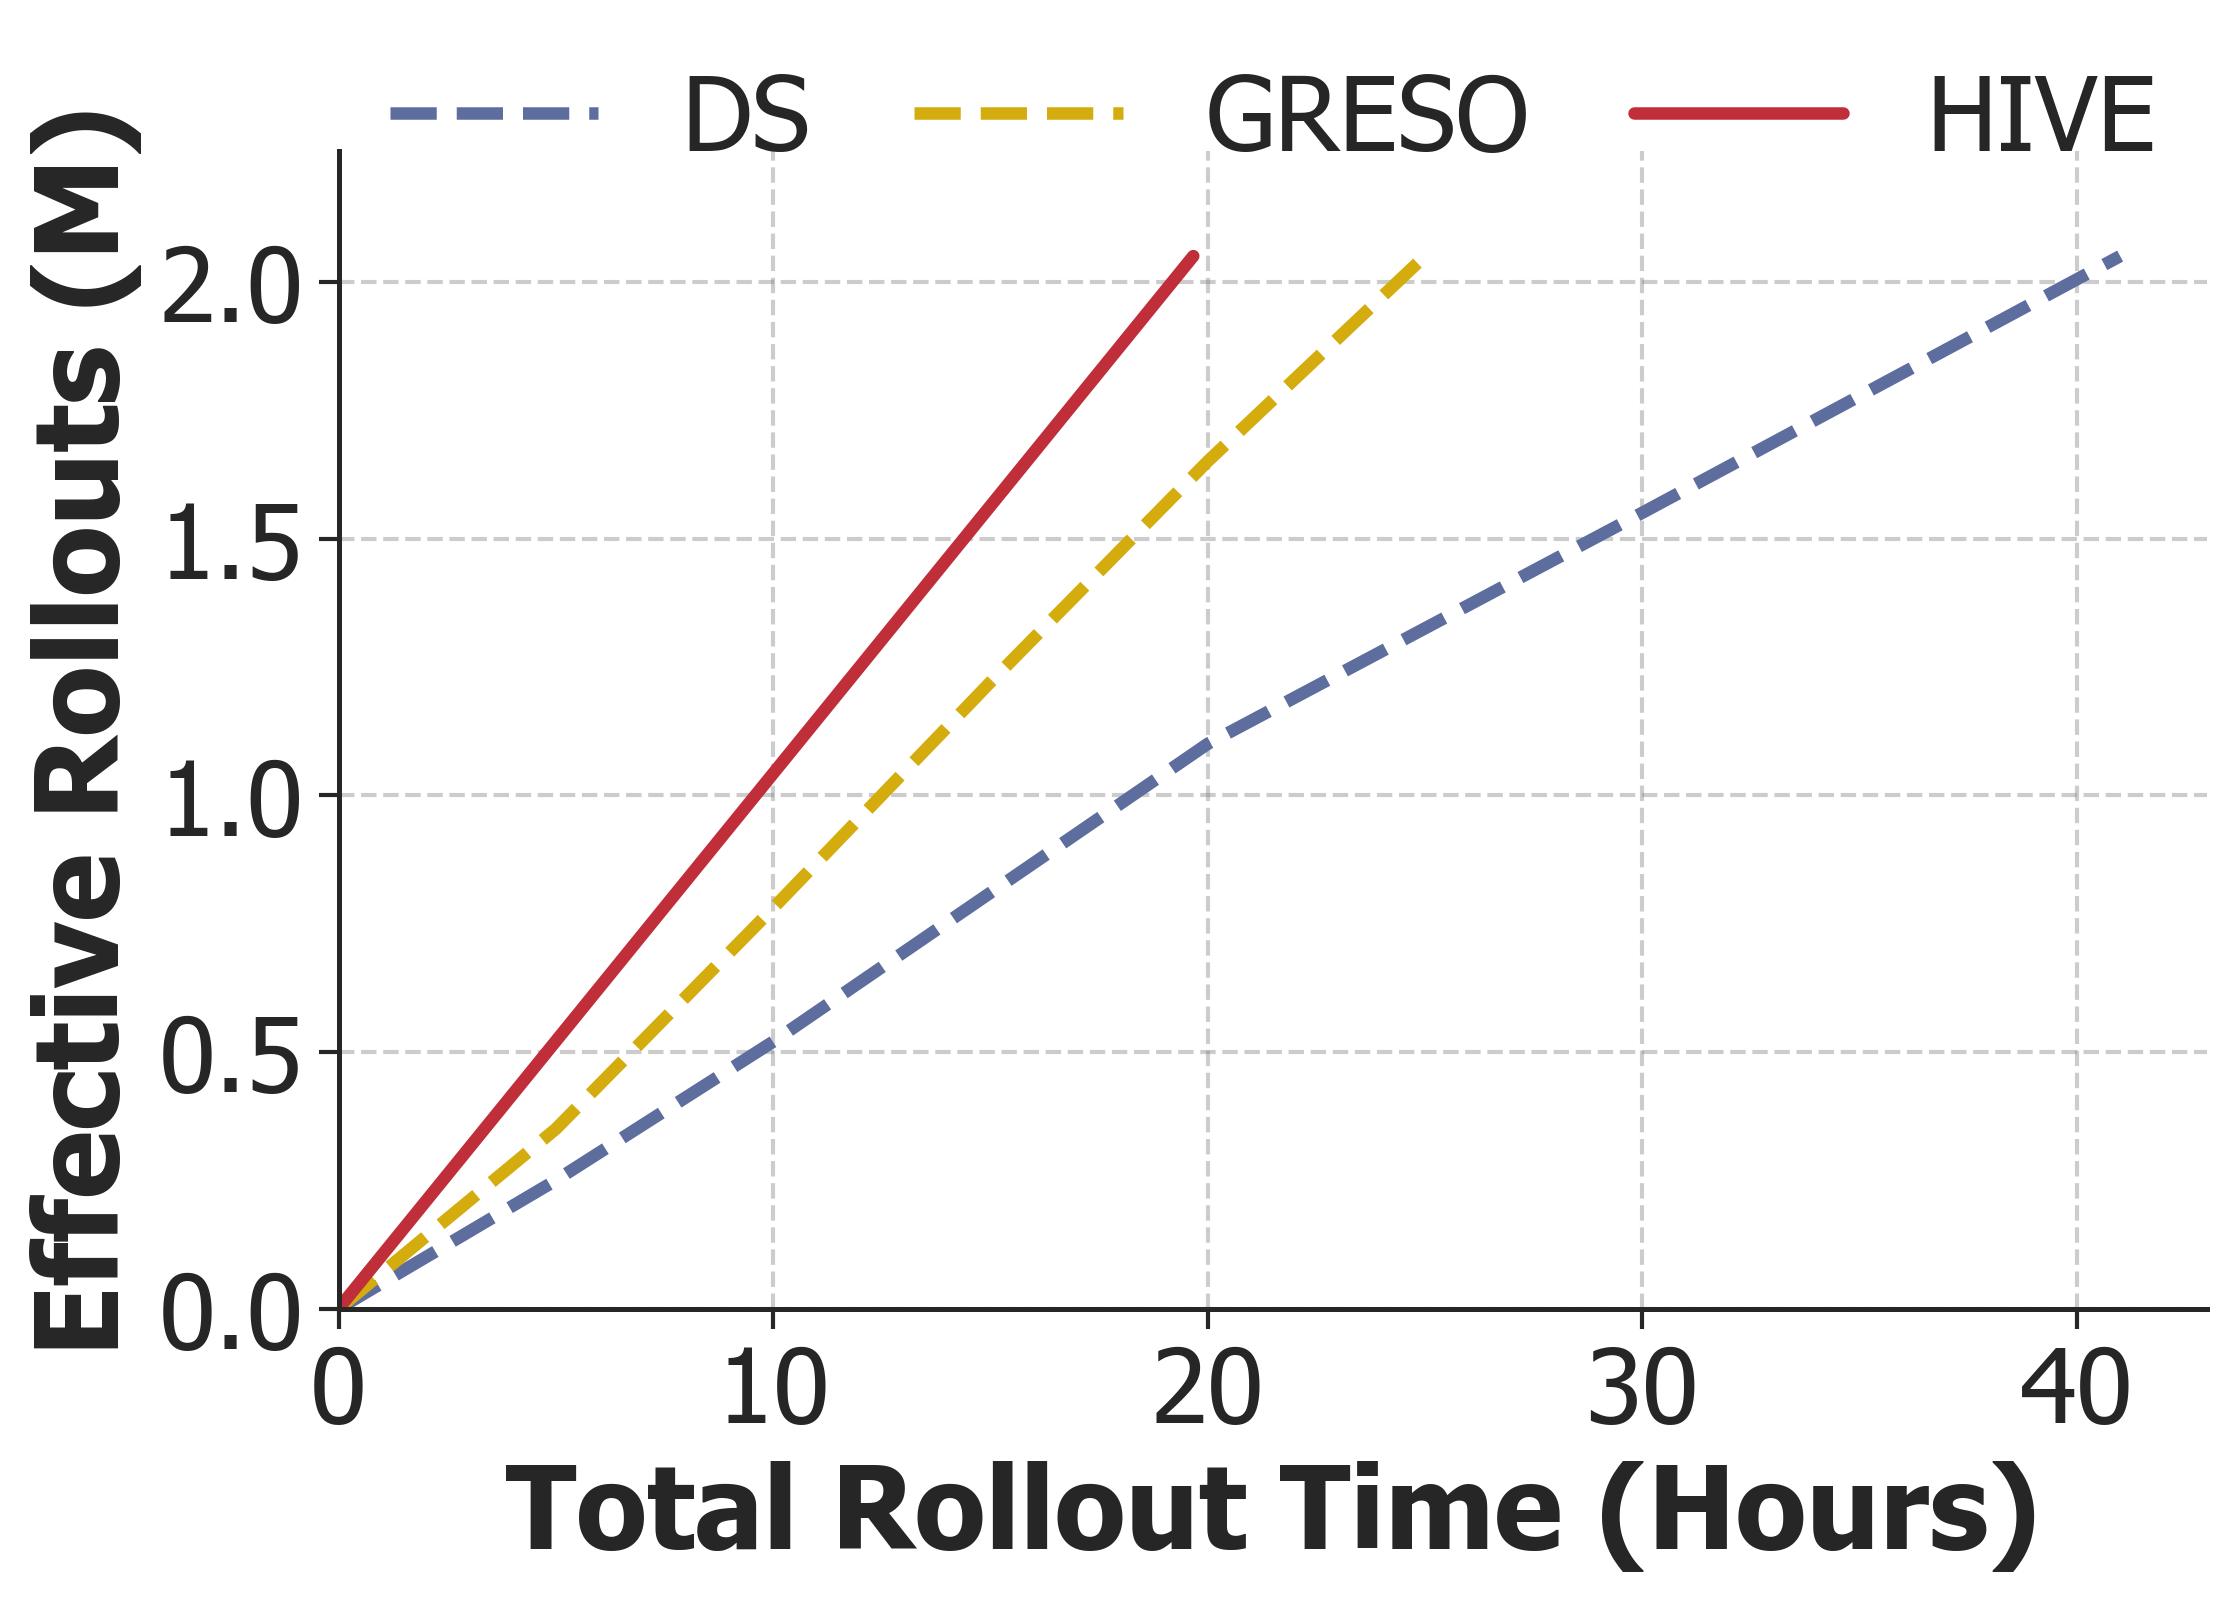
\includegraphics[width=\textwidth]{figures/experiment/11-total-rollout-time-VS-total-effective-rollouts.png}
        \caption{Efficiency Comparison}
        \label{fig:total_rollout}
    \end{subfigure}
    \hfill
    % 第二张图：Generation Time per Step
    \begin{subfigure}[b]{0.24\textwidth}
        \centering
        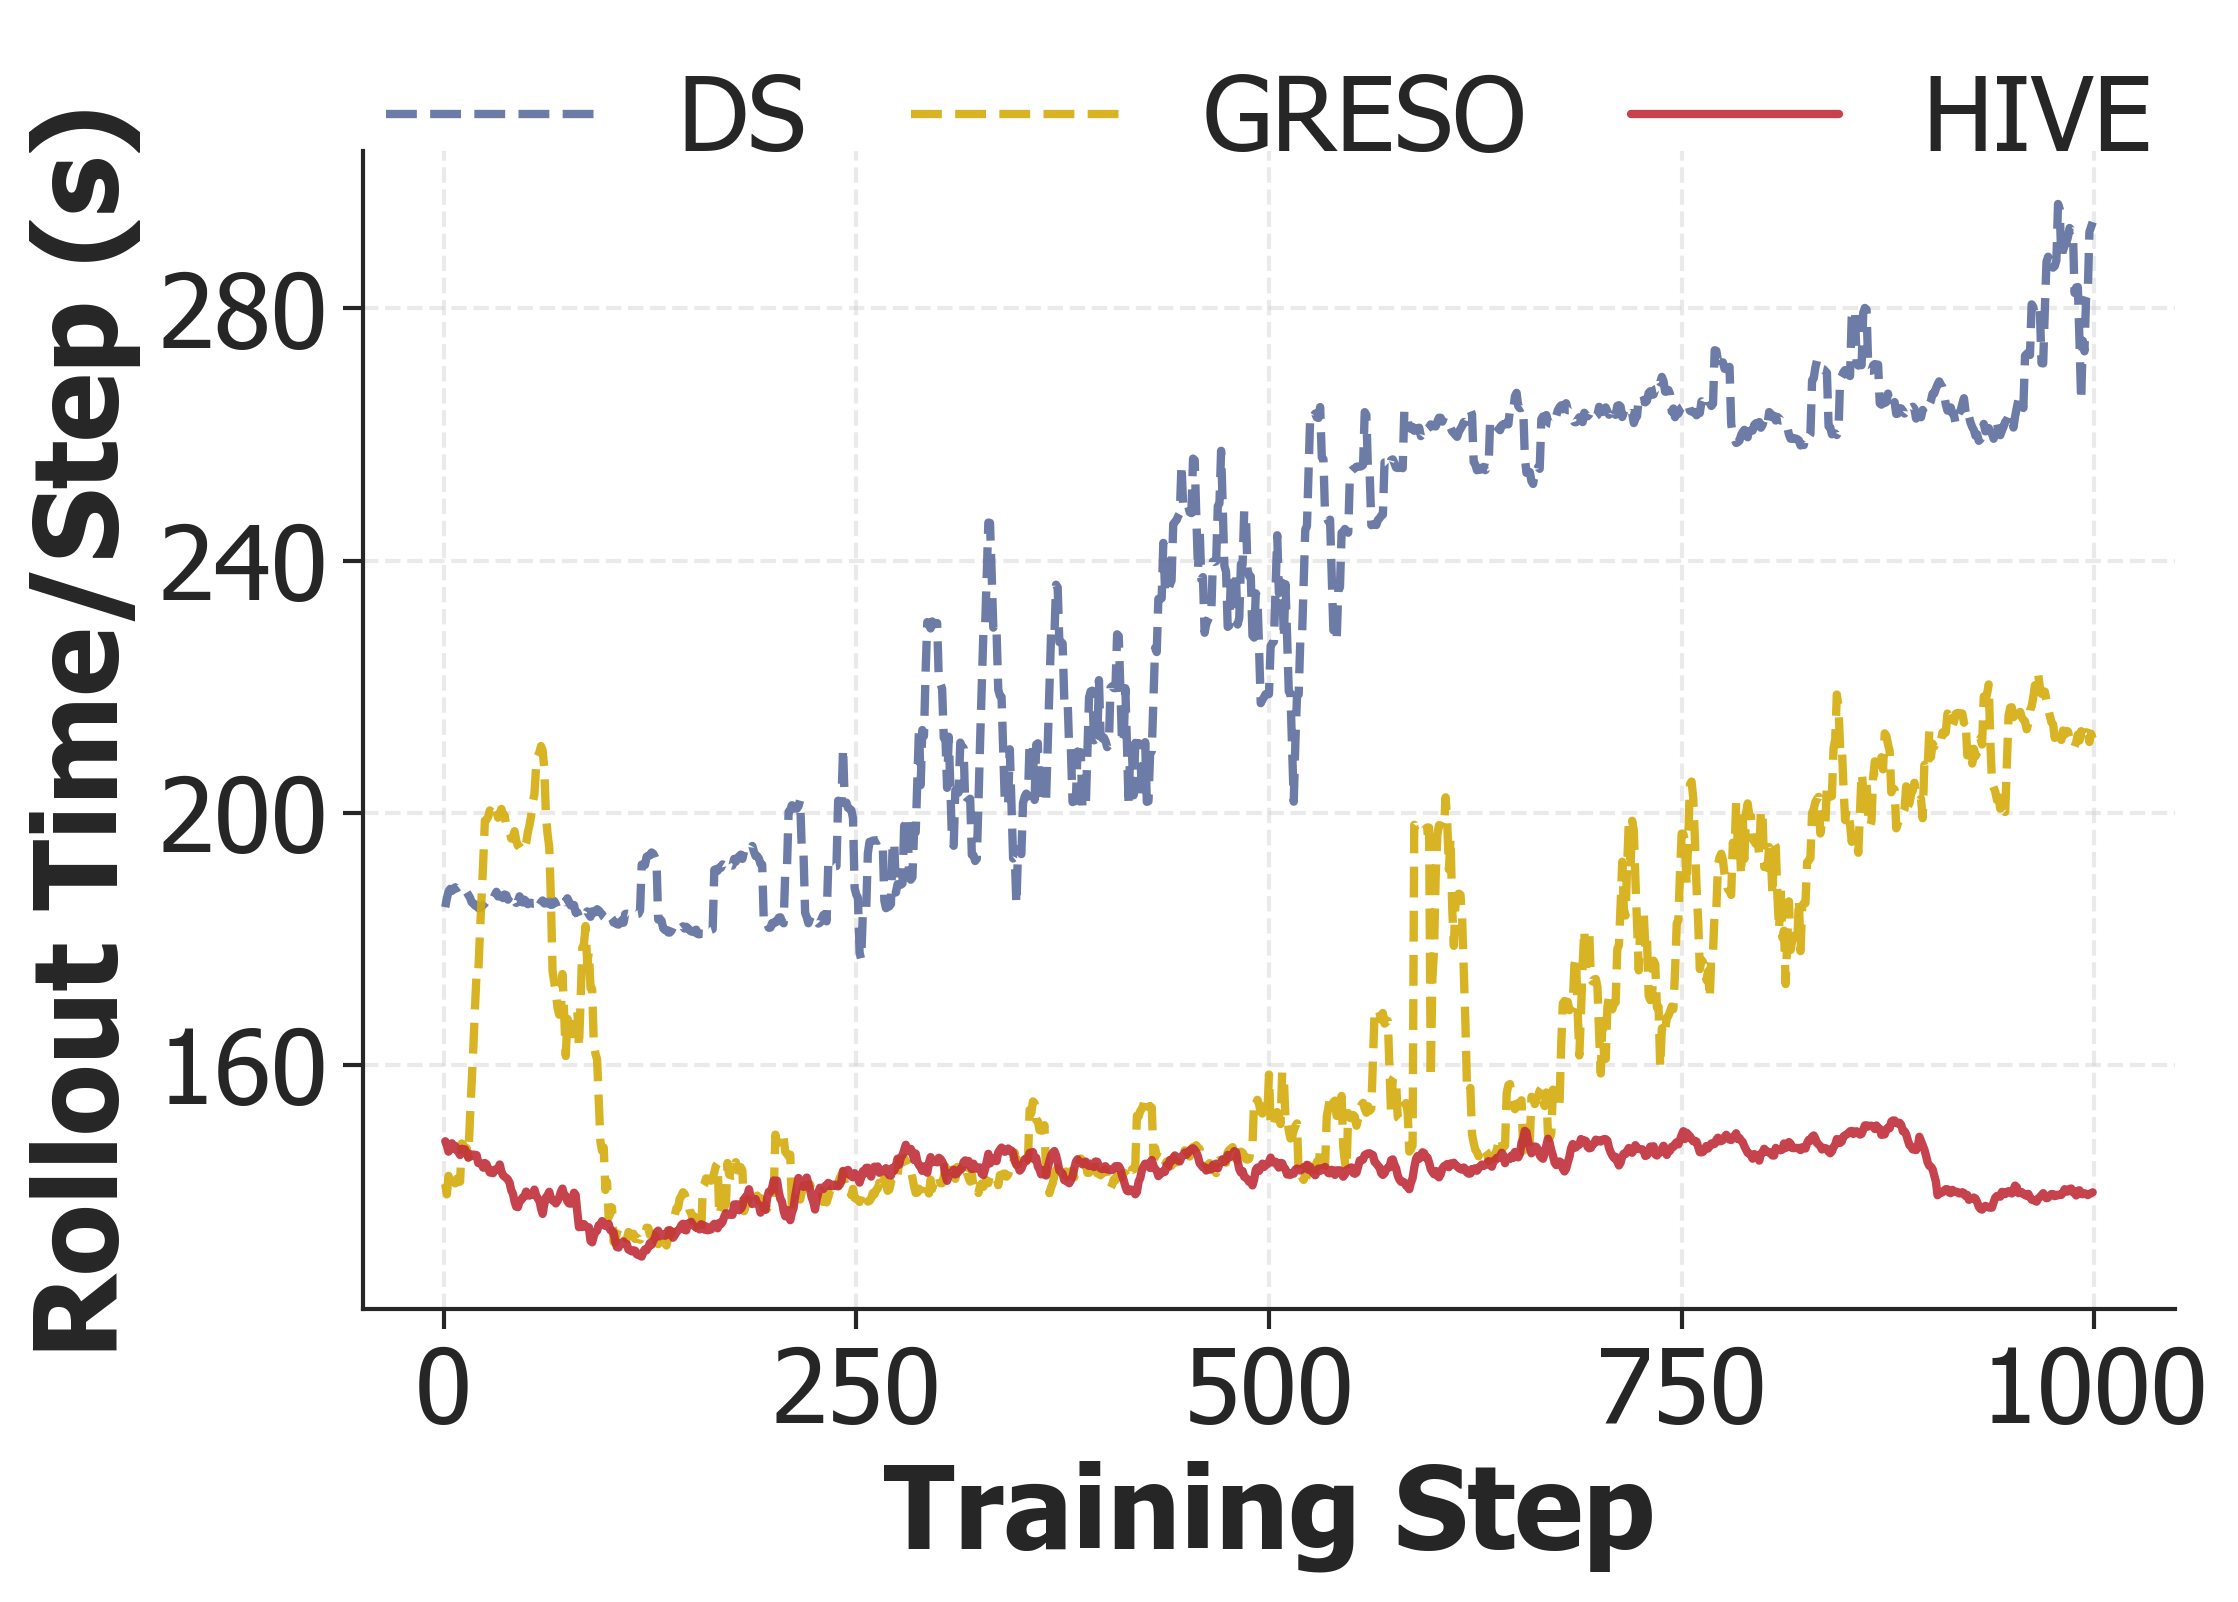
\includegraphics[width=\textwidth]{figures/experiment/10-rollout-time-per-step-comparison-smoothed.png}
        \caption{Generation Time}
        \label{fig:gen_time}
    \end{subfigure}
    \hfill
    % 第三张图：Rollouts per Step
    \begin{subfigure}[b]{0.24\textwidth}
        \centering
        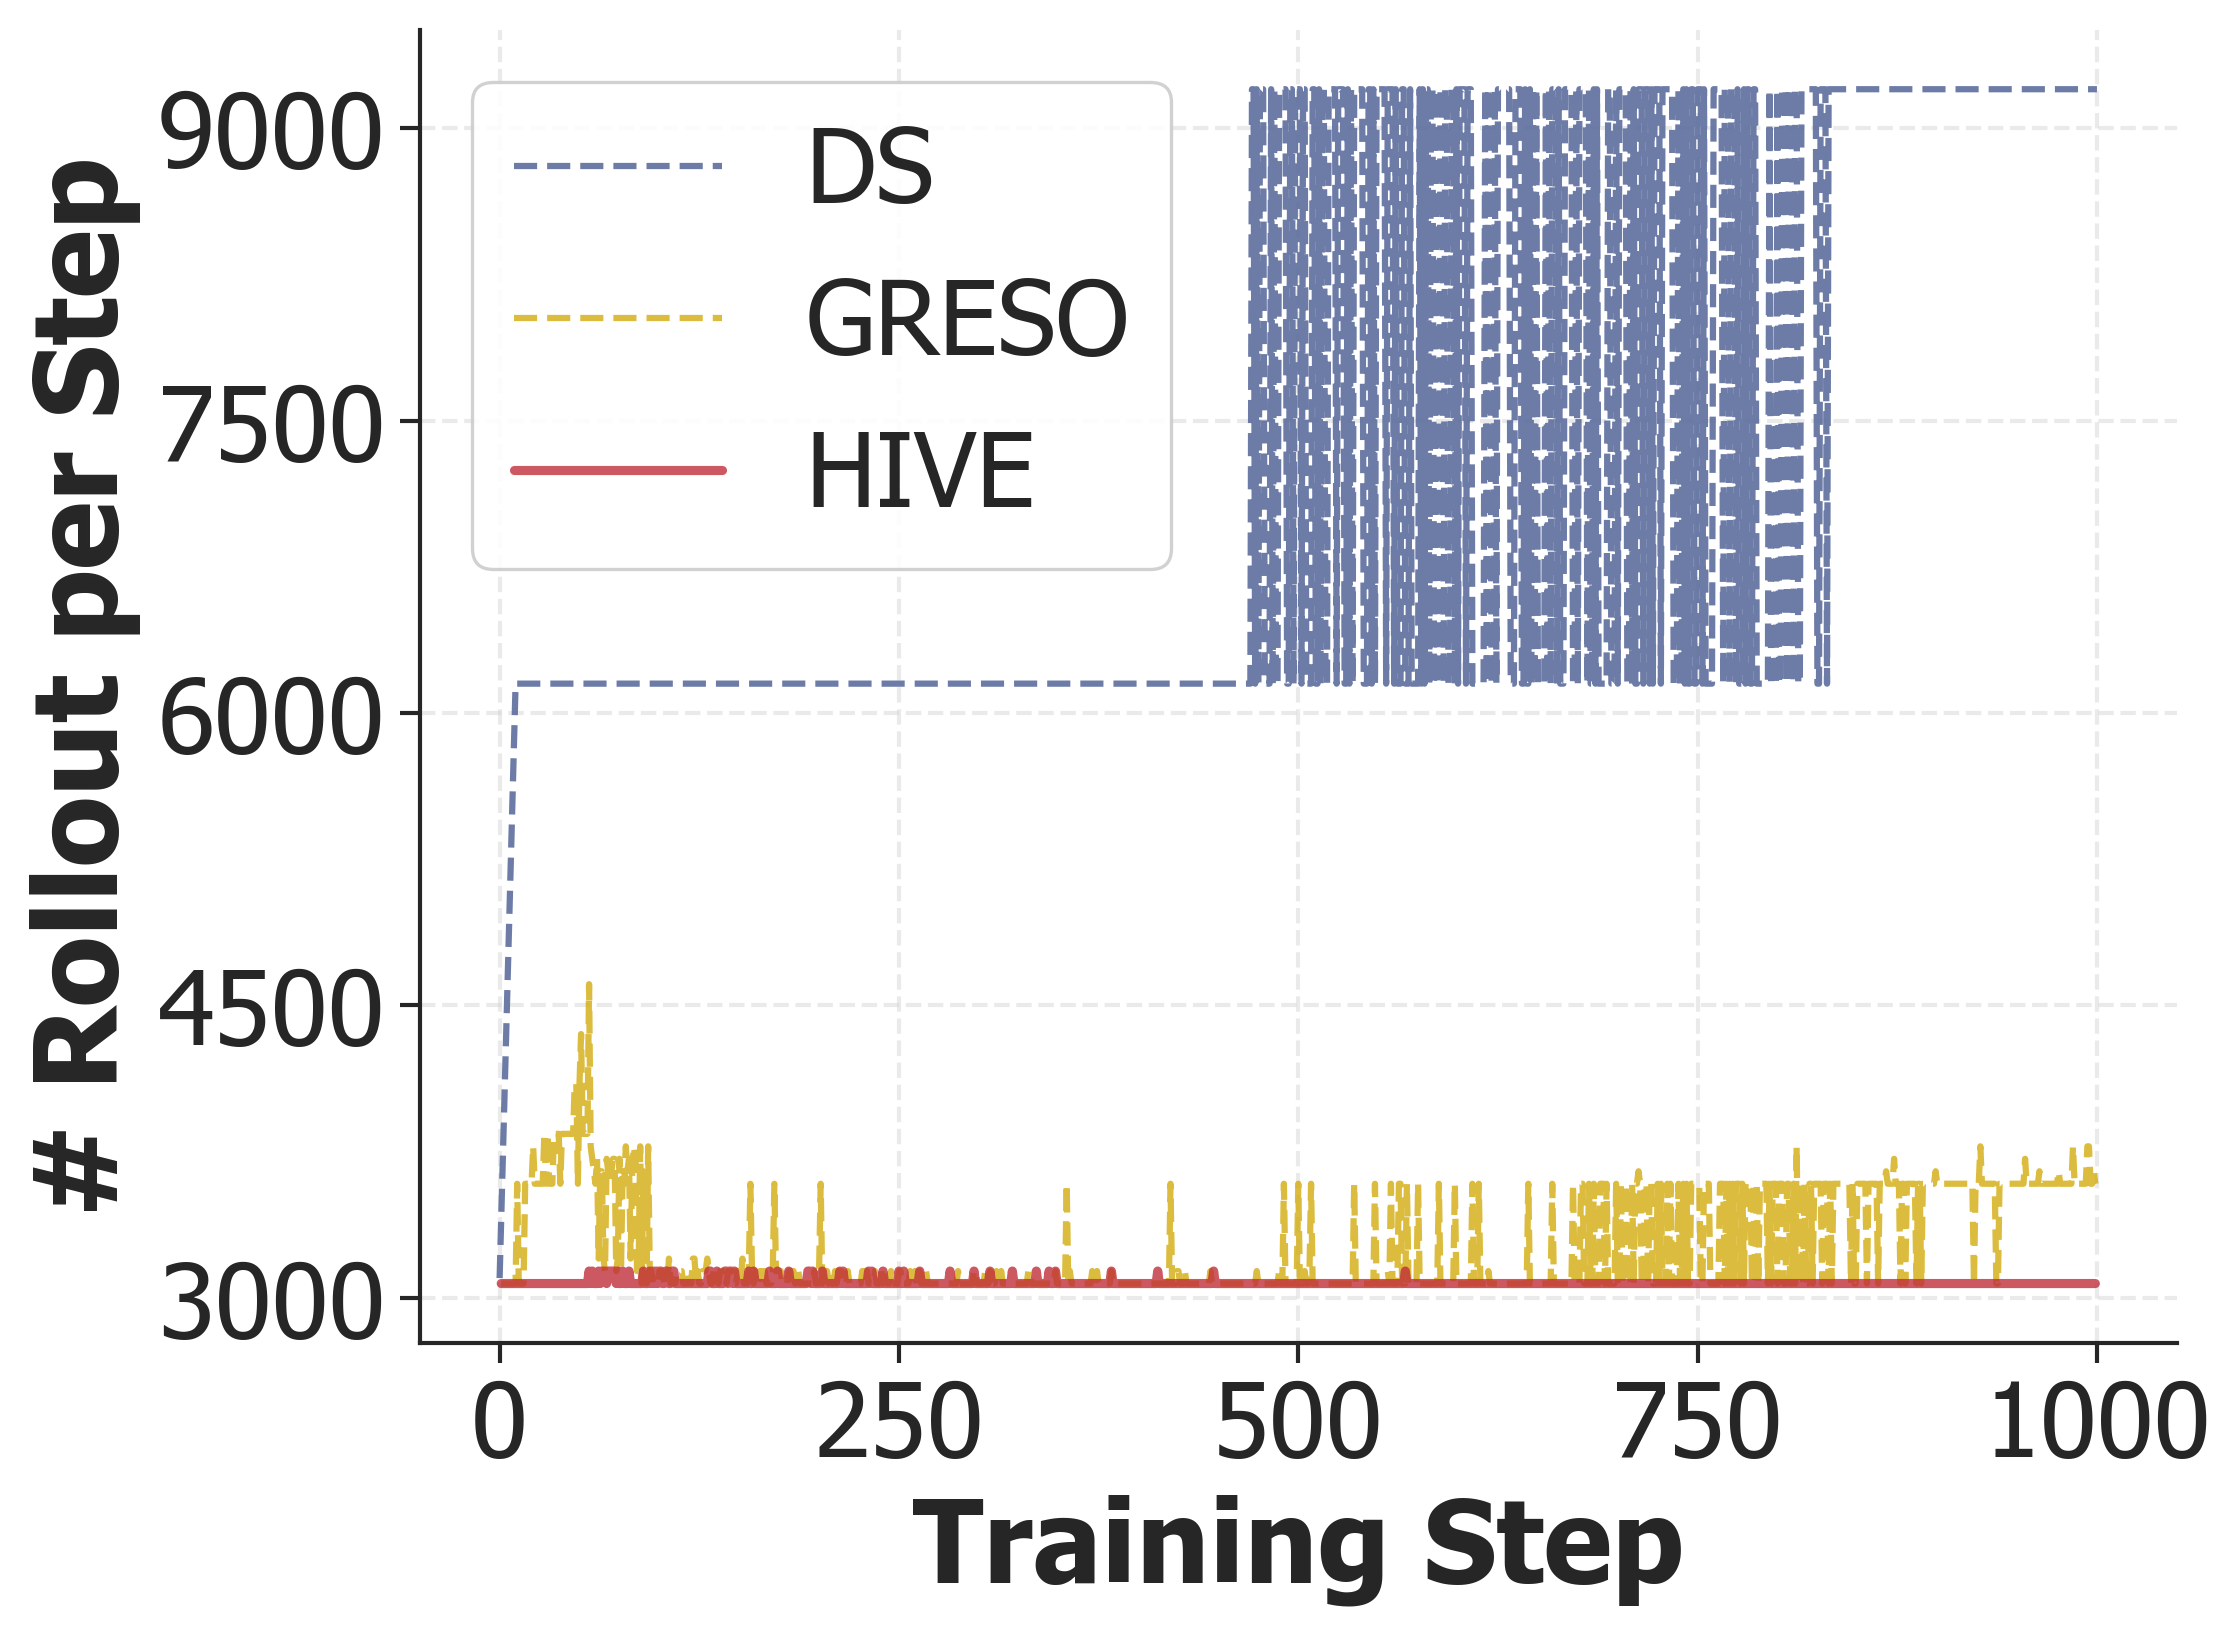
\includegraphics[width=\textwidth]{figures/experiment/8-per-step-rollout-comparison.png}
        \caption{Rollouts per Step}
        \label{fig:rollout_step}
    \end{subfigure}
    \hfill
    
    \caption{Efficiency analysis of Qwen2.5-Math-1.5B trained on DAPO+MATH. (a) Stage~2 prompt-side verification adds little time relative to rollout generation. (b) HIVE accumulates effective rollouts fastest per rollout hour. (c) HIVE maintains lower generation latency throughout training. (d) HIVE rolls out fewer prompt groups per step, concentrating compute on verified candidates.}
    \label{fig:further-analysis}
\end{figure*}
